\chapter{Convolutional Neural Networks}
\label{chapter:intro}
\section{簡介}
卷積神經網路(Convolutional Neural Network)為深度學習的分類模型,是一種前饋神經網路,對於大型圖像處理有出色表現,架構為一層輸入層、數個隱藏層與一層輸出層所組成,其中隱藏層包含有卷積層、池化層與全連接層,分別具有不同的功能。
它與MLP最大的不同點是並非所有神經元會全部連結。
此外訓練過程是從訓練集中以梯度下降法來確定權重與偏差。
\begin{figure}[H]
	\centerline{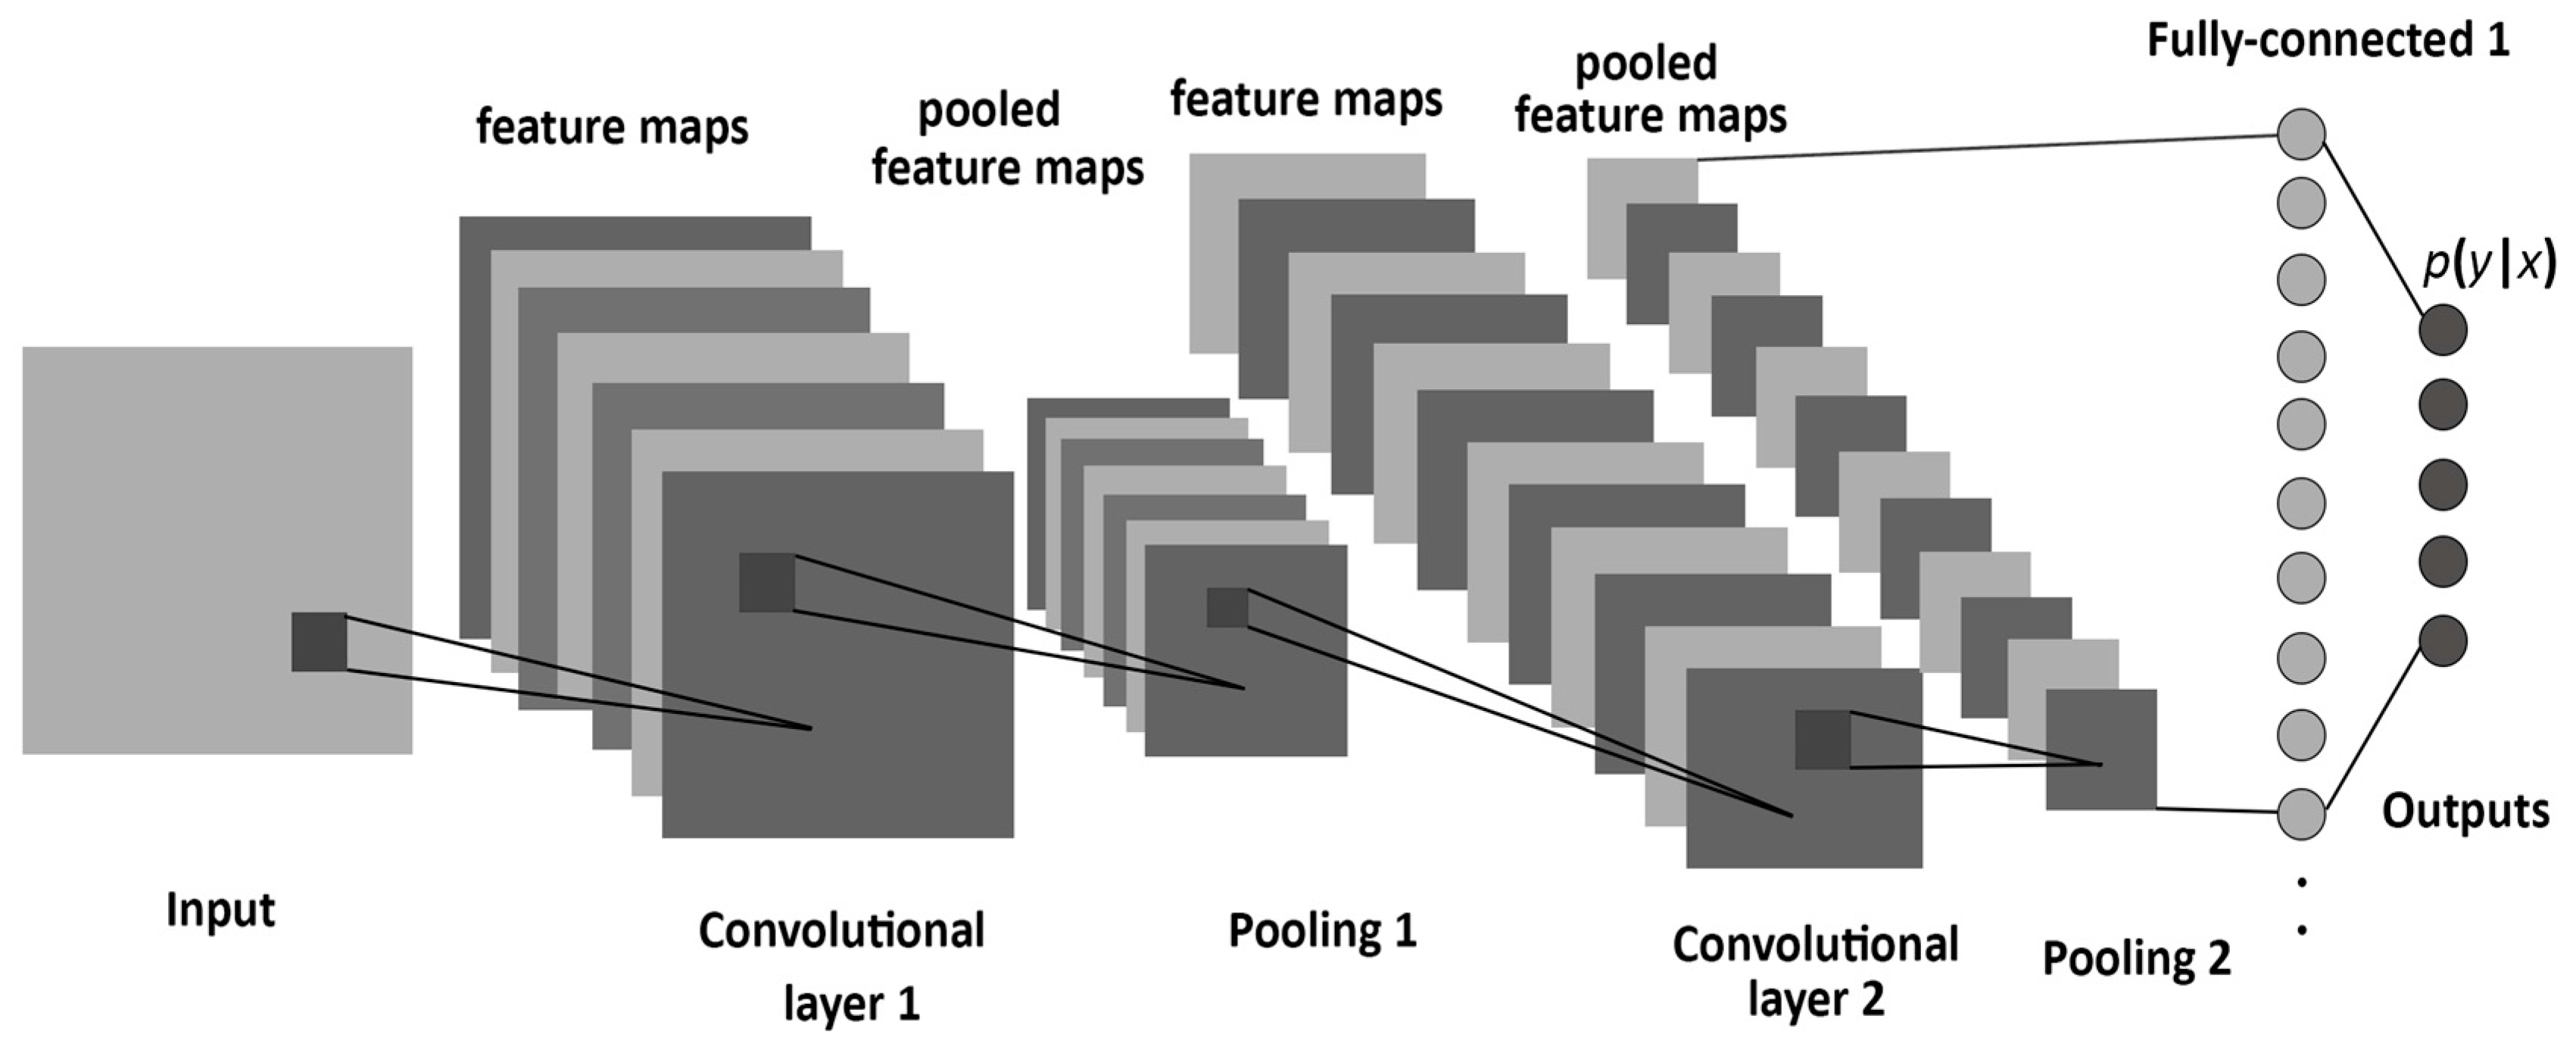
\includegraphics[height=7cm]{pic/CNNAR.png}}
	\caption{CNN架構圖}
	\begin{minipage}{1\linewidth}
		\footnotesize
		\emph{圖片來源:}取自Saleh Albelwi and Ausif Mahmood(2017)。A Framework for Designing the Architectures of Deep Convolutional Neural Networks\end{minipage}

	\label{fig:CNNArchiteture}
\end{figure}


\section{基本結構}
\subsection{輸入層}
輸入層主要的功能用於數據的輸入。
\subsection{卷積層}
\label{subsec:ConvolutionLayer}

在這一層中,主要的目的是進行特徵頡取。CNN是根據影像的特徵來進行分類,不必將整張影像的所有資料點來判別,因為共用相同的特徵參數,如果對上不同影像,只要有相同的特徵出現,就算在不同的區域依然可以找到。圖\ref{fig:Convolution}為卷積的示意圖,利用Mask(圖\ref{fig:Convolution}中藍色區域的部分)在原始影像上移動,再將Kernel Map(圖\ref{fig:Convolution}中黃色區域的部分)的值Mask的值進行內積,這過程稱為卷積(Convolution)。第一格的計算如式(\ref{eqn:ConvolutionCaculate})結果為1,一次往右一格以此類推進行計算,到邊界時往下一列從新的一行開始計算,最後得到Feature Map。

\begin{equation}
	\label{eqn:ConvolutionCaculate}
	2\times(-1)+2\times0+0\times0+0\times0+1\times0+1\times0+0\times1+1\times0+2\times1+1\times1=1
\end{equation}


\begin{figure}[H]
	\centerline{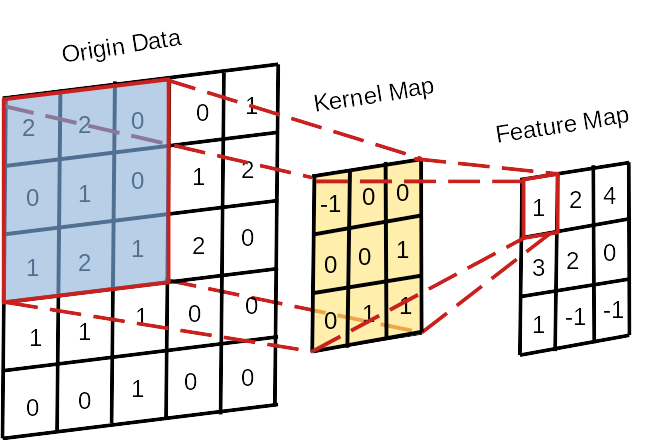
\includegraphics[height=6cm]{./pic/kBPwTe69.png}}
	\caption{卷積示意圖}
	\label{fig:Convolution}
\end{figure}


\newpage
%%具有特徵的濾波器內的權重其數值取得,一開始設置初始權重,因為一開始特徵並不是最好的特徵,因此模型預測與標籤所計算的誤差會非常高。但透過梯度下降法更新濾波器的權重,隨著訓練多次迭代,它會自動趨近於它認為最好的特徵,這特點稱為自動提取特徵。


圖\ref{fig:OriGrayImg}為一張數獨影像,圖\ref{fig:Kernel1Result}與圖\ref{fig:Kernel2Result}為轉換的結果。可以發現原始影像經過Kernel 1萃取後,可提取到水平線的特徵;而經過Kernel 2萃取後,可提取到鉛垂線的特徵。因此,從這個結果可以發現,同一張影像經過不同的Kernel可以萃取到不同的特徵。
\begin{figure}[H]
	\centerline{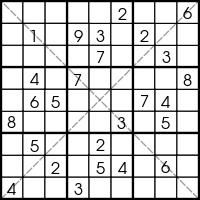
\includegraphics[height=4cm]{pic/gray_img.png}}
	\caption{原始數獨影像}
	\label{fig:OriGrayImg}
\end{figure}


\begin{figure}[H]
	\centerline{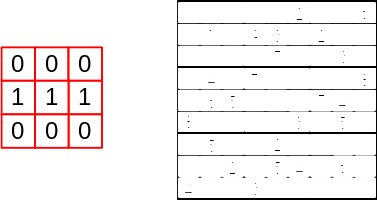
\includegraphics[height=4cm]{./pic/rRdq44Ie.png}}
	\caption{Kernel 1萃取的結果}
	\label{fig:Kernel1Result}
\end{figure}

\begin{figure}[H]
	\centerline{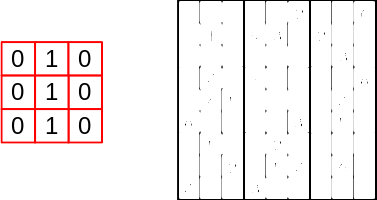
\includegraphics[height=4cm]{./pic/0LHCpsTh.png}}
	\caption{Kernel 2萃取的結果}
	\label{fig:Kernel2Result}
\end{figure}

\begin{comment}
具有特徵提取的Kernel Map,一開始的初值設定在進行特徵提取時,效果並不是很好,因此模型預測與標籤所計算的誤差會非常高。
但透過梯度下降法更新Kernel Map的權重,隨著訓練多次迭代,它會自動趨近於它認為最好的特徵,這特點稱為自動提取特徵。

卷積前後影像大小改變:

是否進填充將影響影像大小的改變,上述例子是採用VALID padding,如圖\ref{fig:Convolution},不在原有的影象基礎上做任何填充,但這樣會有個缺點,在卷積多次後,可能使邊緣的畫素和卷積核做卷積的次數小於影象中間的畫素點,從而導致對其資訊的特徵的提取不足。


所以另一個方法SAME padding,使得做卷積運算後,原始影象的大小會保持原樣。

填充的大小計算公式:
\begin{equation}
	\label{eqn:Padding}
	P=(F-1)/2
\end{equation}

\begin{itemize}
	\item
	      P為填充

	\item
	      F為卷積核的寬 ( 高 ) 度
\end{itemize}


\begin{figure}[H]
	\centerline{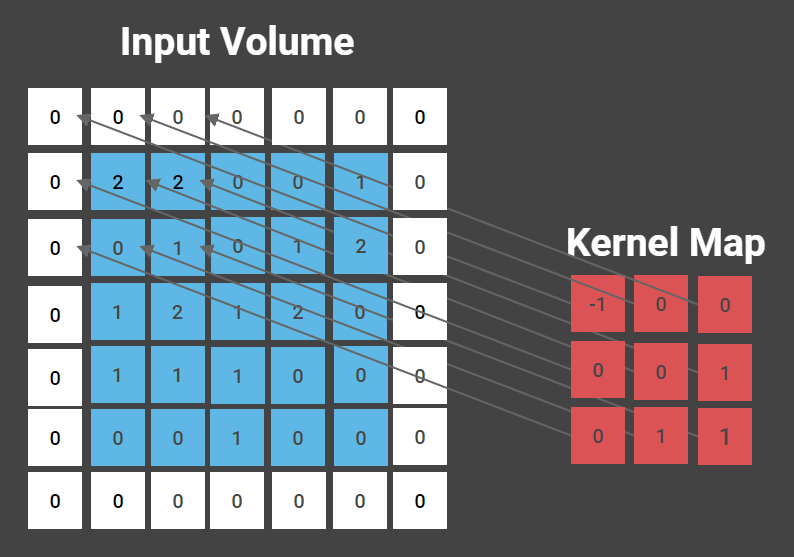
\includegraphics[height=5cm]{pic/samepadding.PNG}}
	\caption{卷積(Convolution)有填充示意圖}
	\label{fig:SamePadding}
\end{figure}
\begin{figure}[H]
	\centerline{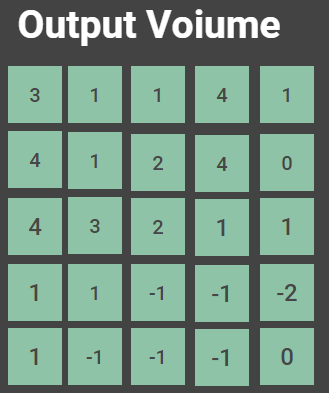
\includegraphics[height=5cm]{pic/samepaddingout.PNG}}
	\caption{卷積(Convolution)有填充結果示意圖}
	\label{fig:SamePaddingOutcome}
\end{figure}


卷積前後影像大小計算:
\begin{equation}
	\label{eqn:ImageShapeAfterConvolution}
	Woutput=(Winput-F+2P)/S+1
\end{equation}

\begin{itemize}
	\item
	      Woutput為特徵圖的寬 ( 高 ) 度
	\item
	      Winput為前圖像寬 ( 高 ) 度
	\item
	      F為卷積核的寬 ( 高 ) 度
	\item
	      P為填充,使用填充:原始影像周圍補上零
	\item
	      S為步長(每次移動遮罩的距離)
\end{itemize}

圖\ref{fig:Convolution}是 \(5 \times5\)的影像,經過\(3 \times 3\)濾波器每次一步,不進行填充卷積後影像為圖\ref{fig:ConvolutionFinally},計算大小(5-3+2*0)/1+1=3,卷積後影像大小為 \(3 \times 3\)


圖\ref{fig:SamePadding}是\(5 \times 5\)的影像經過\(3 \times 3\)濾波器每次一步,進行填充,卷積後影像為圖\ref{fig:SamePaddingOutcome},計算大小(5-3+2*1)/1+1=5,卷積後影像大小為 \(5 \times 5\)

\end{comment}

\subsection{池化層(pooling Layer)}
在這一層中,對影像進行欠取樣(Undersampling),使影像大小在不改變特徵的情況下減少像素,進而達到減少運算的效果,上述方法稱為池化。

池化是先在圖片上選取不同窗口(window),依據不同方法在窗口範圍中選擇特徵值。若使用\(2 \times 2\)的窗口,原圖經過池化以後,其所包含的像素數量會降為原本的四分之一。如圖\ref{fig:MaxPooling}, \(6 \times6\) 的影像經過\(2 \times 2\)的窗口池化後,將變為\(3 \times 3\)的特徵圖,但因為池化後的影像包含了原圖中各範圍的特徵值,並保留每個範圍內各個特徵的相符程度,因此池化後的資訊更專注於影像中是否存在相符的特徵,而非影像中哪裡存在這些特徵。
這能幫助 CNN 判斷圖片中是否包含某項特徵,而不必分心於特徵位置。
目前常見的池化方法有最大池化(Max Pooling)與平均池化(Average Pooling)。

\begin{itemize}
	\item
	      最大池化(Max Pooling):
	      取所有元素的最大值。如圖\ref{fig:MaxPooling}第一個窗口數字為[0.8,0.7,1,0.5] ,進行最大池化後,會選取所有元素的最大值1為特徵值。
	      \begin{figure}[H]
		      \centerline{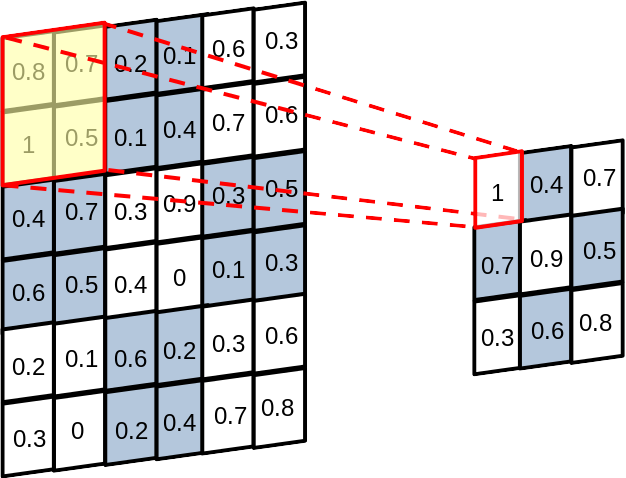
\includegraphics[height=7cm]{./pic/PG7HfVgc.png}}
		      \caption{Max Pooling示意圖}
		      \label{fig:MaxPooling}
	      \end{figure}

	      \newpage
	\item

	      平均池化(Average Pooling):取所有元素的平均值。如圖\ref{fig:AveragePooling}第一個窗口數字為[0.8,0.7,1,0.5] ,經過平均池化,會取所有元素的平均值(0.8+0.7+1+0.5)/4=0.75,作為特徵值。
\end{itemize}

\begin{figure}[H]
	\centerline{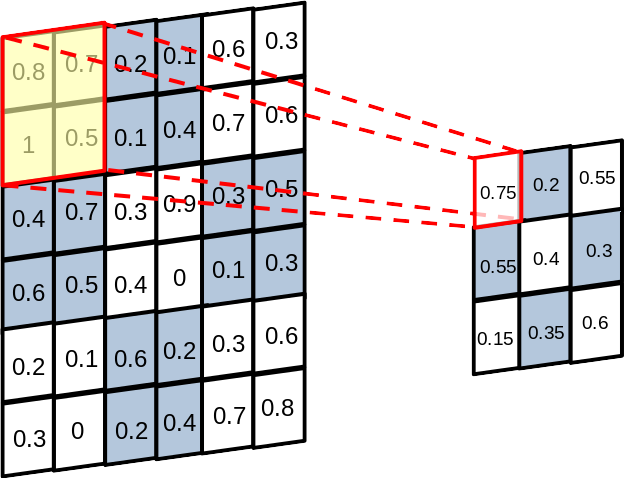
\includegraphics[height=7cm]{./pic/Ec3pr3VH.png}}
	\caption{Average Pooling示意圖}
	\label{fig:AveragePooling}
\end{figure}


圖\ref{fig:Kernel1WithPooling}與圖\ref{fig:Kernel2WithPooling}分別為圖\ref{fig:Kernel1Result}與圖\ref{fig:Kernel2Result},進行 \(2 \times 2\)的 Max Pooling與Average Pooling的結果。從圖中可以發現\(200 \times 200\) 的影像,進行池化後會變為 \(100 \times 100\)的影像,
除此之外,經過池化後的結果,幾乎與原影像的類似,這說明了經過池化不僅可以減少影像的維度,更可以保留原影像的特徵。

\begin{figure}[H]
	\centerline{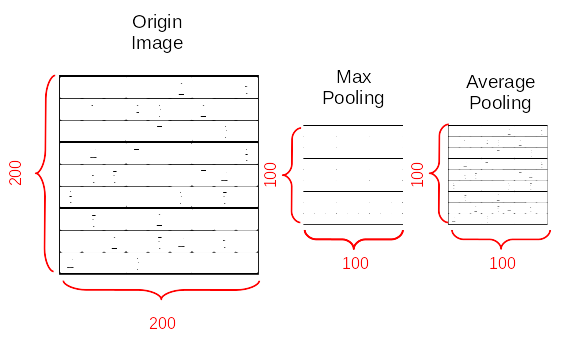
\includegraphics[height=6.5cm]{./pic/iAAoojSF.png}}
	\caption{Average Pooling示意圖}
	\label{fig:Kernel1WithPooling}
\end{figure}

\begin{figure}[H]
	\centerline{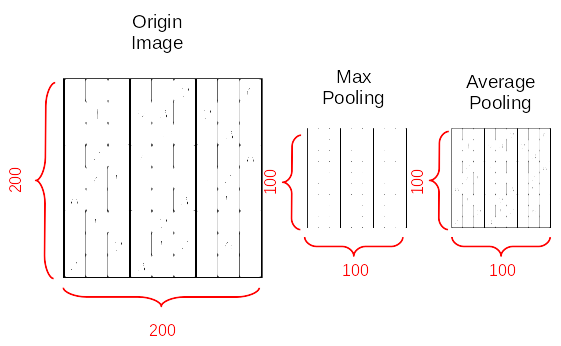
\includegraphics[height=6.5cm]{./pic/f61oy3eL.png}}
	\caption{Average Pooling示意圖}
	\label{fig:Kernel2WithPooling}
\end{figure}

\subsection{全連接層(Fully Connected Layer)}
將所有特徵圖轉為一維度如圖\ref{fig:FullyConnetedLayer},並組合在一起進行輸出分類,換言之就是將數個卷積、池化後的結果進行分類。
通常全連接層與輸出層間會使用Softmax函數(式\ref{eqn:Softmax})輸出各類別的機率。
它能將含任意實數的K維向量「壓縮」至另一個K維實向量中,使得每一個元素的範圍皆位於(0,1)之間,並且所有元素的和為1。

\begin{equation}
	\label{eqn:Softmax}
	\sigma(z)_j=\frac{e^{z_j}}{\sum_{k=1}^{K}e^{zk}} \ \ \ \ \ \ \ \ \ for\ 1,....,K
\end{equation}

\begin{figure}[H]
	\centering
	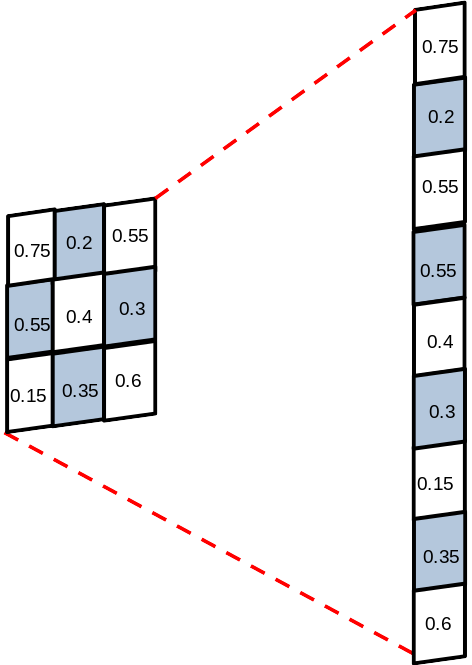
\includegraphics[height=9cm]{./pic/7oVj71cG.png}
	\caption{全連接層示意圖}
	\label{fig:FullyConnetedLayer}
\end{figure}

\section{訓練過程}

\begin{comment}
\subsection{演算法參數}
\begin{lstlisting}[language={python}]
model.add=(Convolution2D(output_size,kernal_size,padding_method,input_shape =(img_channels,img_rows,img_cols))
model.add('activation_function')

\end{lstlisting}

\begin{itemize}
	\item
	      img,輸入圖片。 channels,圖片通道。img rows,img cols:圖片的長寬。
	\item
	      設定卷積核大小Kernal Size(6,6)
	\item
	      output size:卷積後的深度
	\item
	      padding方法:有VALID padding和SAME padding
	\item
	      激活函數使用ReLU函數,式(\ref{eqn:ReLU})
	      \begin{equation}
		      \label{eqn:ReLU}
		      Relu(x)=
		      \left\{\begin{matrix}
			      x \ \ \ \ \ \ if\ x>0
			      \\
			      0 \ \ \ \ \ \ if\ x<0
		      \end{matrix}\right.
	      \end{equation}
\end{itemize}
CNN演算法如圖\ref{fig:Keras}所示
\begin{figure}[H]
	\centerline{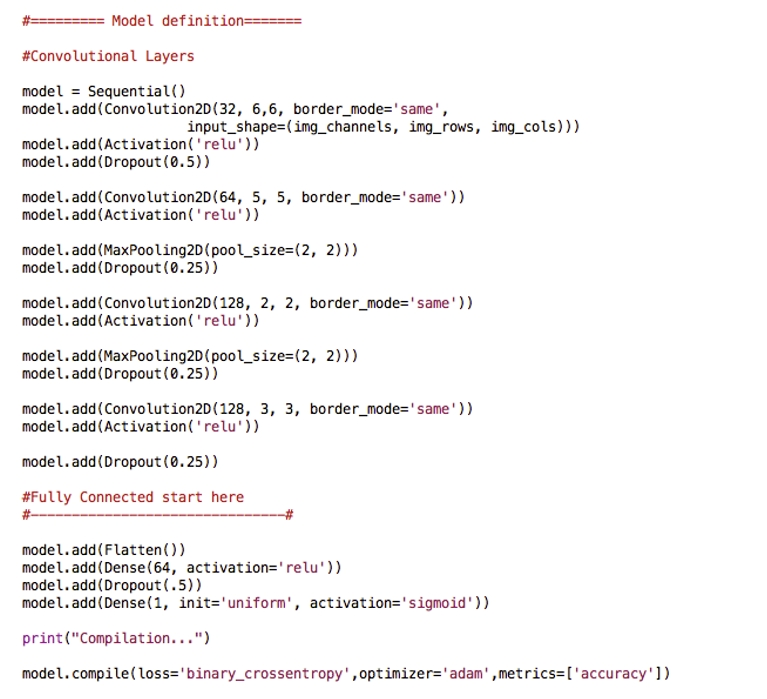
\includegraphics[height=15cm]{pic/Keras.jpg}}
	\caption{CNN演算法圖}
	\label{fig:Keras}
\end{figure}
	
\end{comment}

卷積神經網路的訓練流程如下,圖\ref{fig:CNNTrainningFlowChart}為其訓練流程圖。

\begin{enumerate}
	\item
	      初始化網絡權重。
	\item
	      輸入數據經過卷積層、池化層、全連接層的前向傳播得到輸出值。
	\item
	      求出網絡的輸出值與目標值之間的誤差,判斷是否達到設定的訓練目標。
	\item
	      並將誤差傳回網絡中,反向求得全連接層,池化層,卷積層的誤差。
	\item
	      根據求得誤差進行權重更新,用更新的權重進行回到第二步。
\end{enumerate}
\begin{figure}[H]
	\centerline{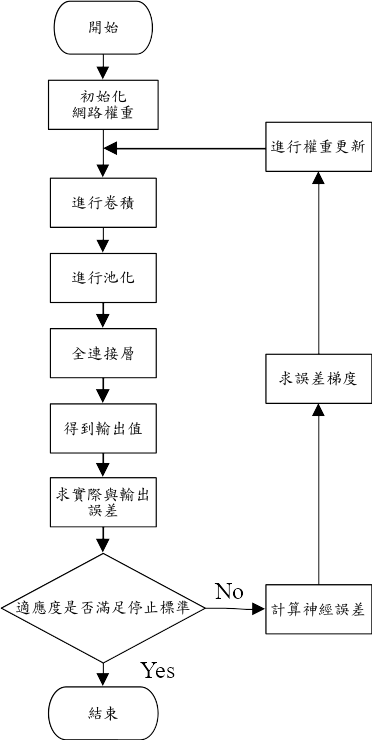
\includegraphics[height=14cm]{./pic/iigz3LNt.png}}
	\caption{CNN訓練流程圖}
	\label{fig:CNNTrainningFlowChart}
\end{figure}

\section{結論}
卷積神經網路利用卷積層進行特徵提取,透過池化層降低維度的同時保留影像特徵,最後經由全連接層進行影像分類的運算。
除此之外,因為卷積神經網路有局部權重共享的特殊性質,能夠降低網路的複雜性,使其在圖形辨識方面有獨特的優勢。

